\documentclass[
	ngerman,
	points=true,% für die Aktivierung der Punktereferenzen funktioniert nicht für TeX Versionen vor 2020
    solution=true,
    accentcolor=9c,
    colorbacktitle
	]{tudaexercise}

\usepackage[english]{babel}
\usepackage[autostyle]{csquotes}
\usepackage{amsmath}
\usepackage{amssymb}
\DeclareMathOperator*{\argmin}{arg\,min}

%Formatierungen für Beispiele in diesem Dokument. Im Allgemeinen nicht notwendig!
\let\file\texttt
\let\code\texttt
\let\pck\textsf
\let\cls\textsf
\let\tbs\textbackslash

\usepackage{booktabs}% Erweiterte möglichkeiten beim Spacing um Linien in Tabellen
\renewcommand*{\creditformatsum}[1]{\creditformat{Gesamt: #1}}

\ConfigureHeadline{
	headline={title-name-id}
}

\begin{document}

\title[Homework 2/4]{Statistical Machine Learning -- Homework}
\author{Prof. Dr. Jan Peters \\ Daniel Palenicek, An Thai Le, Theo Gruner, Maximilian Tölle \& Théo Vincent}
\term{Sommersemester 2023 -- Due date: 05.06.2023, 23:59}
\sheetnumber{2}

\maketitle
Each (sub)task in this homework is worth 1 point. For example, you can get up to 5 points in Task 2.1. The points you achieve in this homework will count towards the exam bonus points. \\
The solutions need to be uploaded to moodle before the deadline. You can provide us with scans of your handwritten solutions or directly write into our .tex file and submit as .pdf. Please make sure that we can exactly determine which solution belongs to which (sub)task. If you decide for handwritten solutions, please understand that we can only give points for answers which we can also read! 

\section*{Density Estimation}
\begin{task}{Parametric Density Estimation}
        \begin{subtask}
        Let's consider an experiment with $K$ different outcomes. The outcomes are modelled as a one-hot encoding
        $$\boldsymbol{x}\in\{0, 1\}^K; \qquad \sum_{i=1}^{K} x_i = 1$$
%

        We chose to model the outcome of the experiment by a random variable $X$ which is distributed as categorical distribution with probability-mass function (pmf) $f(\boldsymbol{x};\boldsymbol{\theta}) = \prod_{i=1}^{K}\theta_i^{x_i}$ where $\theta_i$ represents the probability of $x_i$. Thus, we need to make sure that $\sum_i \theta_i = 1$.
        
        Assume now that we are given a set of data $\mathcal{D} = \{\boldsymbol{x}_j|j=1,\dots,N\}$. Please derive the parameters of the categorical distribution $\theta_i^{\mathrm{ml}}$ that maximize the pmf given the data $\mathcal{D}$.\\
    \end{subtask}
    %
    \begin{solution}
    
    \end{solution}
    \begin{subtask}
        We now consider an experiment where we throw a dice. Which distribution would you choose to model the outcome that we throw a 6. Please state the parameters of your chosen distribution and derive the maximum likelihood parameters. How is your chosen distribution connected to the Categorical distribution?

        Hint: You don't need to run all calculations again to obtain the maximum likelihood parameters.
    \end{subtask}
    \begin{solution}
    
    \end{solution}
    \begin{subtask}\label{subtask:binomial_ml}
        Next up, we consider $n$ throws of the dice. To answer the question how many 6s we can throw with $n$ dices, we model the experiment by a binomial distribution. The random variable $X$ can take values in $x\in\{1,\dots, n\}$ modelling how many times we threw a 6 in $n$ throws. The pmf for the binomial is
        %
        $$f_n(x;\theta) = \begin{pmatrix}
            n\\x
        \end{pmatrix} \theta^{x} (1-\theta)^{n-x}.$$
        %
        Here $n$ denotes the number of trials the experiment is carried out, $x$ denotes the number of times a 6 has been thrown, and $\theta$ is the probability of throwing a 6.
        
        The maximum likelihood estimate of the binomial distribution given a dataset $\mathcal{D}$ can be shown to be
        %
        $$\theta^{\mathrm{ml}} = \frac{1}{N} \sum_{i=1}^{N} \frac{x_i}{n}.$$
        % 
        Please plot the data, collected for $n=10$ throws, provided in \textit{binomial\_data.npy} against the binomial distribution with the maximum likelihood estimate $\theta^{\mathrm{ml}}$ for the $N=10, 100, 1000$ first data points in the dataset. Describe the differences between the three plots.
    \end{subtask}
    \begin{solution}
        
    \end{solution}
    \begin{subtask}
        The beta distribution is a continuous univariate distribution over $\theta$, parameterized by $\alpha$ and $\beta$ with pdf
        %
        \begin{align*}
            \mathrm{beta}(\theta;\alpha, \beta) &= \frac{1}{\mathrm{B}(\alpha, \beta)} \theta^{\alpha - 1}(1-\theta)^{\beta - 1}; \quad \theta\in(0,1)\\
            \mathrm{B}(\alpha, \beta) &= \frac{\Gamma(\alpha)\Gamma(\beta)}{\Gamma(\alpha +  \beta)}
        \end{align*}
        %
        Here $\mathrm{B}(\alpha, \beta)$ is the beta-function, represented by the gamma-function, which acts as a normalization constant. The term is not required for the further calculations and thus, we will not further introduce it.

        Let's assume that the parameters of the binomial likelihood $\mathrm{binomial}_n(x|\theta)$ in sub-task~\ref{subtask:binomial_ml} are random variables. We define the prior over the parameters by a beta distribution with $\alpha_0$, $\beta_0$. Calculate the posterior of the likelihood under the beta prior. Which type of distribution does the posterior assume? How is this concept called in the literature?

        Hint: Please elaborate if you need to explicitly calculate the evidence? Use the fact that the posterior is proportional to the joint distribution.
        \end{subtask}
        \begin{solution}
            
        \end{solution}
        \begin{subtask}
            In Bayesian inference the posterior is updated sequentially by adding more and more data. Please plot the prior distribution, with $\alpha_0 = \beta_0 = 1$, and the posterior distribution $p(\theta|x_{1:N})$ for the first $N=1,2,5,10,100$ datapoints. Use the results of the previous question. Also plot the maximum likelihood estimate of the binomial distribution for $N=1000$ datapoints from sub-task~\ref{subtask:binomial_ml}. Interpret the results and outline the differences between Bayesian estimation and maximum likelihood estimation.
        \end{subtask}
    \begin{solution}
        
    \end{solution}
\end{task}

\begin{task}{Non-Parametric Density Estimation}

Given the following dataset graph

\begin{center}
    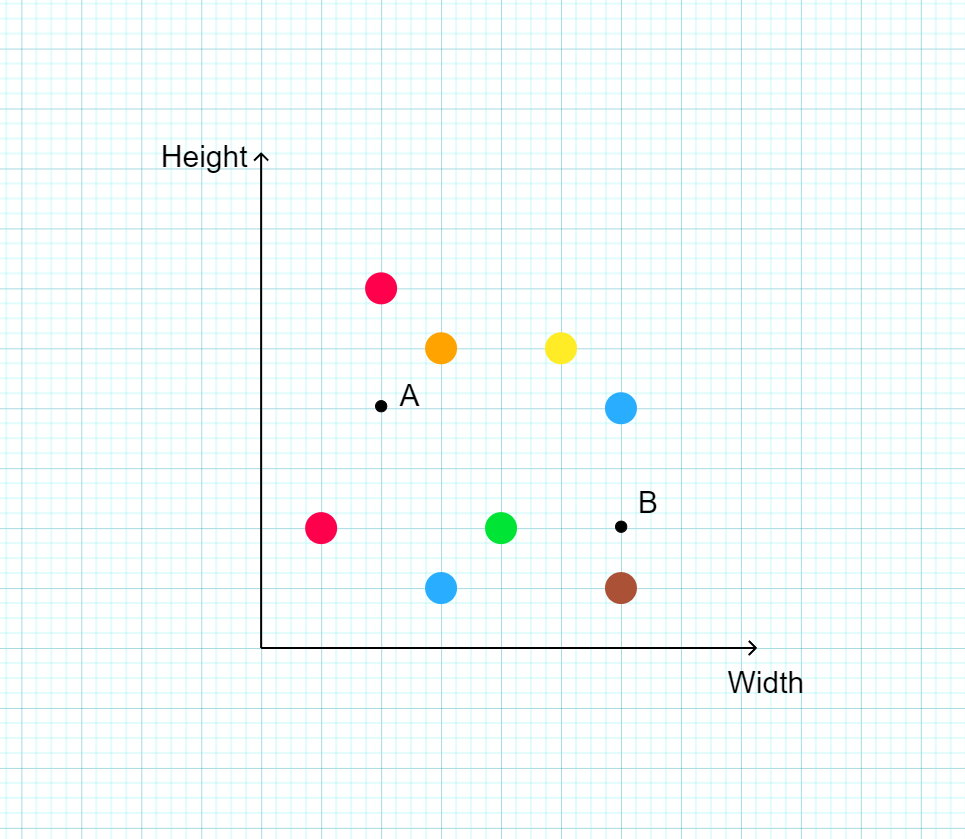
\includegraphics[width=0.6\textwidth]{figures/non_parametric_ex.png}
    % \caption{Fruit dataset graph. }
    \label{fig:fruit}
\end{center}

depicting the fruit colors (Red, Orange, Blue, Green, Yellow, and Brown) with their corresponding width and height features. For example, the Brown fruit has the (width, height) value of (6, 1). We consider using k-Nearest Neighbor (kNN) method to classify the colors of the fruit A and B depicted in the graph, utilizing a kernel to quantify the similarity between the data points. Let us define the Euclidean distance $d(\boldsymbol{x}, \boldsymbol{y}) = \left\| \boldsymbol{x} - \boldsymbol{y}\right\|$ to define distance on the feature space of width and height. We choose the parameter $k = 3$.

\begin{subtask}

Assuming the kernel is the inverse of the squared distance  $k(\boldsymbol{x}, \boldsymbol{y}) = \frac{1}{d(\boldsymbol{x}, \boldsymbol{y})^2}$, classify the color of fruit A and B.
    
\end{subtask}

\begin{subtask}

Assuming the kernel is Gaussian $k(\boldsymbol{x}, \boldsymbol{y}) = e^{-\alpha d(\boldsymbol{x}, \boldsymbol{y})^2}$, classify the color of fruit A and B in both cases $\alpha=0.2$. What is the problem when we set $\alpha = 20$ or higher?
    
\end{subtask}
    
\end{task}

\newpage

\section*{Clustering \& Evaluation}
\begin{task}{EM Algorithm and K-Means}
In this task, we would like to find groups of similar data points through the use of clustering algorithms. If not stated otherwise, please assume the most general case of having $N$ data points of dimensionality $D$ that can be grouped into $K$ clusters. \\
\textbf{Note:} As this task puts great emphasis on the implementation of clustering algorithms, please provide all your python code with explanatory comments where needed. 
\begin{subtask}
Derive the update equations of the maximization step of the EM algorithm as introduced in the lecture. Start by writing down the log-likelihood function of a multivariate Gaussian mixture distribution. \\
\textbf{Hint:} For the derivation of the update equation for the mixing coefficients $\pi_k$, consider the constraint $\sum_{k=1}^{K}\pi_k=1$. 
\end{subtask}
\begin{solution}

\end{solution}

\begin{subtask}
Using python, implement the EM algorithm from scratch by writing one function for each of the following steps:
\begin{itemize}
    \item expectation step
    \item maximization step
    \item log likelihood estimation.
\end{itemize}
Afterwards, implement the main function of the EM algorithm which leverages the previously implemented functions. As the stopping criterion, check if the log likelihood has converged, i.e. the absolute difference in subsequent values is below a certain threshold $\epsilon$. You do not need to care about the initialization yet. 
\end{subtask}
\begin{solution}
    
\end{solution}

\begin{subtask}
As mentioned in the lecture, it is often necessary to introduce a regularization for EM with GMM to make sure that no singularities occur in the estimation. Using python, implement the function that adds a small value to the diagonal entries of all covariance matrices, i.e. $\boldsymbol{\Sigma}_{\text{reg}}=\boldsymbol{\Sigma}+\sigma_{\text{min}}\boldsymbol{I}$. Add this function to your EM algorithm. Why does this problem not arise for a single Gaussian distribution when maximizing its log likelihood function over $n>1$ data points? 
\end{subtask}
\begin{solution}
    
\end{solution}

\begin{subtask}
We also know from the lecture that the EM algorithm is sensitive to its initialization and beyond that computationally expensive. Therefore, we would like to initialize the means and the covariances of the Gaussian Mixture Model with clustering results of the K-Means algorithm. The K-Means algorithm should run for a certain number of iterations before its results are used for initialization. \\
Please implement the K-Means algorithm. The obtained cluster centers should be used as the initial means. The covariance matrices of the GMM should be initialized as $\boldsymbol{\Sigma}_{\text{init, k}}=\sigma_{\text{init, k}}\boldsymbol{I}$ where $\sigma_{\text{init, k}}$ corresponds to the mean of the squared euclidean distances between the kth cluster mean and corresponding associated data points. \\ 
Initialize the mixing coefficients $\pi_k$ uniformly over all $K$ components. 
\end{subtask}
\begin{solution}
    
\end{solution}

\begin{subtask}
We now want to test the implemented algorithm on the provided dataset $clustering\_dataset.npy$. As it is typical in machine learning, you need to think about good initial parameter values as well as good hyperparameters. Please explain your choices. \\ What is the maximum log likelihood that you have obtained with your best fitted model? Please visualize your final clustering result and the corresponding GMM. Create a table for the initialization values of K-Means and EM, the chosen hyperparameters of both algorithms and the means, covariances and mixing coefficients of the GMM.
\end{subtask}
\begin{solution}
    
\end{solution}

\begin{subtask}
Often, the data space is not arranged in a simple manner. Please explain if the EM-GMM algorithm can correctly group the following data points into 2 clusters.
\begin{center}
    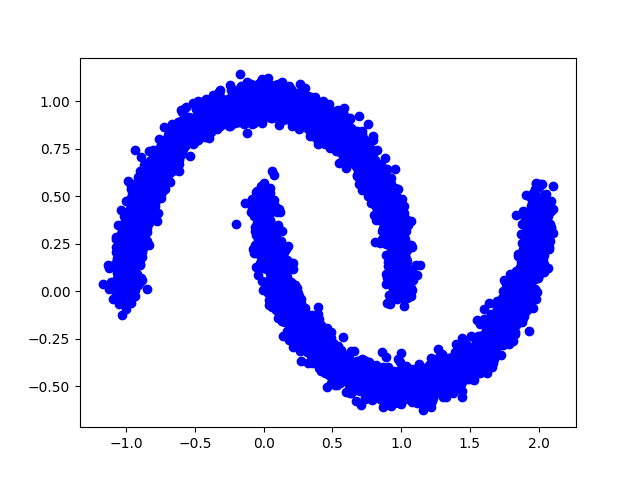
\includegraphics[scale=0.5]{figures/clustering_moons.png}
\end{center}
\end{subtask}
\begin{solution}
    
\end{solution}
\end{task}

\begin{task}{Bias \& Variance}
\begin{subtask}
In the lecture, it has been claimed that the maximum likelihood estimation of the variance of a Gaussian distribution is biased. Please proof this statement by deriving the corresponding bias term.
\end{subtask}
\begin{solution}
    
\end{solution}

\begin{subtask}
It has further been claimed that we can obtain an unbiased estimator. Please derive the corrected variance estimate.
\end{subtask}

\begin{solution}
    
\end{solution}

\begin{subtask}
Typically, there is a tradeoff between bias and variance. Please explain the concept using the example of the mean shift clustering algorithm. 
\end{subtask}
\begin{solution}
    
\end{solution}

\end{task}

\newpage

\section*{Classification}
\begin{task}{Perceptron algorithm}
We consider a classification problem where we want to find the decision boundary determining two classes ($\mathcal{C}_1$ and $\mathcal{C}_2$) using the perceptron algorithm.
\begin{subtask}
Write the objective function to maximize knowing that a member of $\mathcal{C}_1$ is correctly classified if the Perceptron discriminant function equals to $1$.
\end{subtask}
\begin{solution}

\end{solution}

\begin{subtask}
Compute the gradient of the objective function and use it to explain how the pseudo-code of the Perceptron algorithm introduced in the slide 44/61 is built. Focus on the lines:
\begin{itemize}
    \item If $\boldsymbol{x}_{i}$ is correctly classified, i.e., $y\left(\boldsymbol{x}_{i}\right)=y_{i}$, do nothing
    \item Else if $y_{i}=1$ update the parameters with
    $$
    \boldsymbol{w}\leftarrow\boldsymbol{w}+\boldsymbol{x}_{i},\quad b\leftarrow b+1
    $$
    \item Else if $y_{i}=-1$ update the parameters with
    $$
    \boldsymbol{w}\leftarrow\boldsymbol{w}-\boldsymbol{x}_{i},\quad b\leftarrow b-1
    $$
\end{itemize}
\end{subtask}
\begin{solution}

\end{solution}

\begin{subtask}
In practice, the stopping criterion of the \textit{for} loop is not used since there is no guarantee that the algorithm converges. Instead, the stopping criterion is based on a pre-defined number of iterations. Additionally, the points of the dataset are taken randomly. Here is how the pseudo-code looks like:
\begin{itemize}
    \item Initialize the weight vector $\boldsymbol{w}$ and bias $b$ to zero.
    \item For $n$ iterations
    \begin{itemize}
        \item select an index $i$ uniformly at random
        \item If the data point $\boldsymbol{x}_{i}$ is correctly classified, i.e., $y\left(\boldsymbol{x}_{i}\right)=y_{i}$, do nothing
        \item Else if $y_{i}=1$ update the parameters with
        $$
        \boldsymbol{w}\leftarrow\boldsymbol{w}+\boldsymbol{x}_{i},\quad b\leftarrow b+1
        $$
        \item Else if $y_{i}=-1$ update the parameters with
        $$
        \boldsymbol{w}\leftarrow\boldsymbol{w}-\boldsymbol{x}_{i},\quad b\leftarrow b-1
        $$
    \end{itemize}
\end{itemize}

Using Python, code the Perceptron algorithm to determine a decision boundary with $n = 1000$. You can find the dataset in two files: \textit{data.npy} and \textit{labels.npy}. The file \textit{data.npy} contains a matrix representing the dataset of the points to classify. It is composed of $50$ points of $2$ dimensions. The file \textit{labels.npy} contains the list of labels. The first element of this list is the label of the first point in \textit{data.npy} and so on... You can load the \textit{.npy} file with the function \textit{numpy.load}.

We expect you to answer with a plot showing the decision boundary along with the dataset. Comment on the obtained solution. Please, include your code in the answer, which should not exceed $40$ lines.
\end{subtask}
\begin{solution}

\end{solution}

\begin{subtask}
With Python, run the Perceptron algorithm to determine a decision boundary with $n = 1000$ using the same dataset as the previous question. However, this time, we ask you to pre-process the dataset to compute features before running the Perceptron algorithm. For a point $\begin{bmatrix} x \\ y \end{bmatrix}$, please use the following feature representation: $\begin{bmatrix} x \cos(y) \\ x \sin(y) \end{bmatrix}$. 

We expect you to answer with a plot showing the decision boundary along with the dataset. Comment on the obtained solution. Please, include your code in the answer, which should not exceed $40$ lines.
\end{subtask}
\begin{solution}

\end{solution}

\begin{subtask}
With Python, run only the first iteration ($n = 1$) of the \textit{for} loop of the Perceptron algorithm with $i=5$ to determine a decision boundary using the same dataset as the previous question.

We expect you to answer with a plot showing the decision boundary along with the dataset. Please use a different marker for the only point taken into account by the algorithm (the $5^{\text{th}}$ one). Comment on the obtained solution. Please, include your code in the answer, which should not exceed $40$ lines.
\end{subtask}
\begin{solution}

\end{solution}
\end{task}

\end{document}